\documentclass[journal,12pt,onecolumn]{IEEEtran}
\usepackage{graphicx, float}
\graphicspath{{Figs/}}
\usepackage{multicol}
\usepackage{parskip}
\usepackage{titlesec}
\usepackage{color}
\usepackage{enumitem}
\usepackage{amsmath,amssymb,amsfonts,amsthm}
\usepackage{array}
\usepackage{booktabs}
\usepackage[table]{xcolor}
\usepackage{longtable}
\usepackage{gensymb}
\usepackage{cite}
\usepackage{algorithmic}
\usepackage{textcomp}
\usepackage{txfonts}
\usepackage{listings}
\usepackage{mathtools}
\usepackage{comment}
\usepackage{tkz-euclide}
\usepackage[breaklinks=true]{hyperref}
\usepackage{gvv}
\usepackage[utf8]{inputenc}
\usetikzlibrary{arrows.meta, positioning}
\usepackage{xparse}
\usepackage{calc}
\usepackage{multirow}
\usepackage{hhline}
\usepackage{ifthen}
\usepackage{lscape}
\usepackage{tabularx}

\begin{document}

\title{
ASSIGNMENT 1: GATE 2014 \\
BT: AGRICULTURAL ENGINEERING}
\author{AI25BTECH11025-R Nikhil}
\maketitle
\renewcommand{\thefigure}{\theenumi}
\renewcommand{\thetable}{\theenumi}


\title{GATE 2014 -- AGRICULTURAL ENGINEERING (AG)}
\date{}
\maketitle




\begin{enumerate}
    \item Choose the most appropriate word from the options given below to complete the following sentence.

    A person suffering from Alzheimer’s disease ------- short-term memory loss.
    \begin{multicols}{2}
    \begin{enumerate}
        \item experienced
        \item has experienced
        \item is experiencing
        \item experiences
    \end{enumerate}
    \end{multicols}
    \hfill(GATE AG 2014)

    \item Choose the most appropriate word from the options given below to complete the following sentence

    ------- is the key to their happiness; they are satisfied with what they have.
    \begin{multicols}{4}
    \begin{enumerate}
        \item Contentment
        \item Ambition
        \item Perseverance
        \item Hunger
    \end{enumerate}
    \end{multicols}
    \hfill(GATE AG 2014)

    \item Which of the following options is the closest in meaning to the sentence below?

    “As a woman, I have no country.”
    \begin{enumerate}
        \item Women have no country.
        \item Women are not citizens of any country.
        \item Women’s solidarity knows no national boundaries.
        \item Women of all countries have equal legal rights.
    \end{enumerate}
    \hfill(GATE AG 2014)

    \item In any given year, the probability of an earthquake greater than Magnitude 6 occurring in the Garhwal Himalayas is 0.04. The average time between successive occurrences of such earthquakes is --------- years.

    \hfill(GATE AG 2014)

    \item The population of a new city is 5 million and is growing at 20\% annually. How many years would it take to double at this growth rate?
    \begin{multicols}{4}
    \begin{enumerate}
        \item 3-4 years
        \item 4-5 years
        \item 5-6 years
        \item 6-7 years
    \end{enumerate}
    \end{multicols}
    \hfill(GATE AG 2014)

    \item In a group of four children, Som is younger to Riaz. Shiv is elder to Ansu. Ansu is youngest in the group. Which of the following statements is/are required to find the eldest child in the group?
    Statements
    
    1. Shiv is younger to Riaz.
    
    2. Shiv is elder to Som.
    \begin{enumerate}
        \item Statement 1 by itself determines the eldest child.
        \item Statement 2 by itself determines the eldest child.
        \item Statements 1 and 2 are both required to determine the eldest child.
        \item Statements 1 and 2 are not sufficient to determine the eldest child.
    \end{enumerate}
    \hfill(GATE AG 2014)

\item Moving into a world of big data will require us to change our thinking about the merits of exactitude. 
To apply the conventional mindset of measurement to the digital, connected world of the twenty-first century 
is to miss a crucial point. As mentioned earlier, the obsession with exactness is an artefact of the 
information-deprived analog era. When data was sparse, every data point was critical, and thus great care was 
taken to avoid letting any point bias the analysis.  

\textit{From ``BIG DATA'' Viktor Mayer-Schonberger and Kenneth Cukier}  

\medskip
The \textbf{main} point of the paragraph is:

    \begin{enumerate}
        \item The twenty-first century is a digital world
        \item Big data is obsessed with exactness
        \item Exactitude is not critical in dealing with big data
        \item Sparse data leads to a bias in the analysis
    \end{enumerate}
    \hfill(GATE AG 2014)

    \item The total exports and revenues from the exports of a country are given in the two pie charts below.
    The pie chart for exports shows the quantity of each item as a percentage of the total quantity of exports. The pie chart for the revenues shows the percentage of the total revenue generated through export of each item. The total quantity of exports of all the items is 5 lakh tonnes and the total revenues are 250 crore rupees. What is the ratio of the revenue generated through export of Item 1 per kilogram to the revenue generated through export of Item 4 per kilogram?
    \begin{figure}[H]
        \centering
        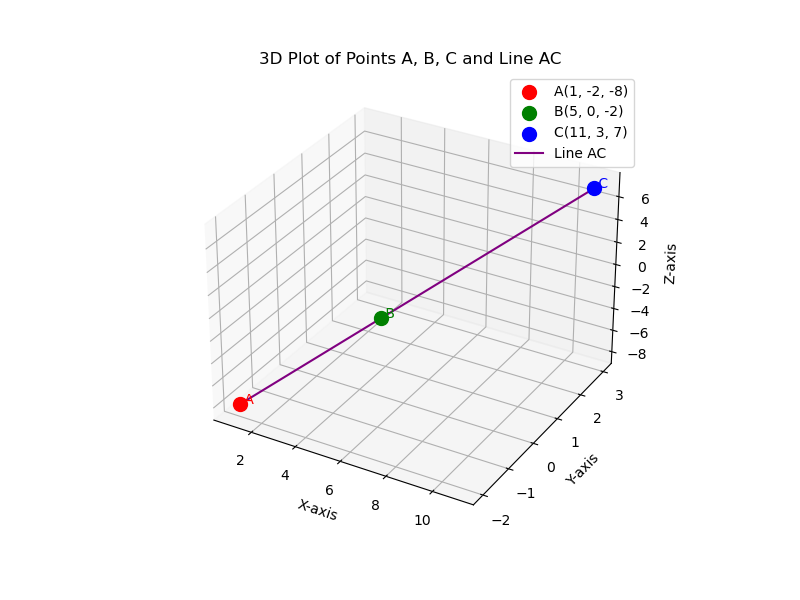
\includegraphics[width=0.8\textwidth]{Fig.png}
        \caption{}
        \label{fig:Q8}
    \end{figure}
    \begin{multicols}{4}
    \begin{enumerate}
        \item 1:2
        \item 2:1
        \item 1:4
        \item 4:1
    \end{enumerate}
    \end{multicols}
    \hfill(GATE AG 2014)

    \item X is 1 km northeast of Y. Y is 1 km southeast of Z. W is 1 km west of Z. P is 1 km south of W. Q is 1 km east of P. What is the distance between X and Q in km?
    \begin{multicols}{4}
    \begin{enumerate}
        \item 1
        \item $\sqrt{2}$
        \item $\sqrt{3}$
        \item 2
    \end{enumerate}
    \end{multicols}
    \hfill(GATE AG 2014)

    \item 10\% of the population in a town is HIV$^+$. A new diagnostic kit for HIV detection is available; this kit correctly identifies HIV$^+$ individuals 95\% of the time, and HIV$^-$ individuals 89\% of the time. A particular patient is tested using this kit and is found to be positive. The probability that the individual is actually positive is \\\\\\.

    \hfill(GATE AG 2014)

    \item If two independent variables $X$ and $Y$ are uncorrelated then
    \begin{multicols}{2}
    \begin{enumerate}
        \item $Cov(X,Y) = 0$
        \item $Cov(X,Y) > 0$
        \item $Cov(X,Y) < 0$
        \item $-1 < Cov(X,Y) < 1$
    \end{enumerate}
    \end{multicols}
    \hfill(GATE AG 2014)

    \item A partial differential equation containing dependent variable $u$ is given by
    \[A \frac{\partial^2 u}{\partial x^2} + 2B \frac{\partial^2 u}{\partial x \partial y} + C \frac{\partial^2 u}{\partial y^2} + D \frac{\partial u}{\partial x} + E \frac{\partial u}{\partial y} + F u + G = 0\]
    where $A, B, C, D, E, F$ and $G$ are constants or functions of independent variables $x$ or $y$ only. Also $G \neq 0$. The nature of the equation is
    \begin{multicols}{2}
    \begin{enumerate}
        \item Linear and homogeneous
        \item Non-linear and homogeneous
        \item Linear and non-homogeneous
        \item Non-linear and non-homogeneous
    \end{enumerate}
    \end{multicols}
    \hfill(GATE AG 2014)

    \item If $f(x,y) = 3x^2 - 4xy + 2y^2$, the summation of $\frac{\partial f}{\partial x}$ and $\frac{\partial f}{\partial y}$ for $x = 1$ and $y = 2$ is \\\\\\.

    \hfill(GATE AG 2014)

    \item The brake power of a four-cylinder engine is 30 kW with all cylinders firing and 20 kW with any one cylinder cut. The mechanical efficiency of the engine in percent is
    \begin{multicols}{4}
    \begin{enumerate}
        \item $60$
        \item $67$
        \item $75$
        \item $83$
    \end{enumerate}
    \end{multicols}
    \hfill(GATE AG 2014)

    \item A tractor is provided with an Ackerman steering gear mechanism. If $b$ is the wheel base, $c$ the distance between the front wheel pivot points, $\theta$ the steering angle of the inner wheel and $\phi$ the steering angle of the outer wheel, the fundamental relationship to be satisfied to avoid skidding of the two front wheels during a turn is given by
    \begin{enumerate}
        \item $\tan \phi - \tan \theta = \frac{c}{b}$
        \item $\cot \phi - \cot \theta = \frac{c}{b}$
        \item $\tan \theta - \tan \phi = \frac{b}{c}$
        \item $\cot \phi - \cot \theta = \frac{b}{c}$
    \end{enumerate}
    \hfill(GATE AG 2014)

    \item Match the processes given in Group-I with the derived products given in Group-II.
    \begin{table}[H]
    \begin{tabular}{cc}
        Group-I & Group-II \\
        i. Transesterification & a. Producer gas \\
        ii. Pyrolysis & b. Ethanol \\
        iii. Yeast fermentation & c. Biogas \\
        iv. Anaerobic digestion & d. Biodiesel \\
    \end{tabular}
    \caption{}
    \label{table match the following}
    \end{table}
    \begin{enumerate}
        \item i-a; ii-c; iii-b; iv-d
        \item i-d; ii-c; iii-b; iv-a
        \item i-b; ii-d; iii-a; iv-c
        \item i-d; ii-a; iii-b; iv-c
    \end{enumerate}
    \hfill(GATE AG 2014)

    \item While operating a pedal thresher, 14 kg of paddy seed remained unthreshed for a throughput of 112 kg. If the quantity of the threshed seed obtained was 70 kg, the threshing efficiency in percent is
    \begin{multicols}{4}
    \begin{enumerate}
        \item $62.50$
        \item $80.00$
        \item $83.33$
        \item $87.50$
    \end{enumerate}
    \end{multicols}
    \hfill(GATE AG 2014)

    \item The pitch of the chain used in a chain drive motion is 38 mm. If the number of teeth on one of the sprockets is 35, the pitch circle diameter of the sprocket in m is -------.

    \hfill(GATE AG 2014)

    \item A tractor tyre contains 31 L of air at a pressure of 190 kPa and a temperature of 30$^\circ$C. Using R=8.314 J (gmol)$^{-1}$ K$^{-1}$ and molecular mass of air = 29 g (gmol)$^{-1}$, the mass of air contained in the tyre is $M \times 10^{-3}$ kg. The value of $M$ is --------.

    \hfill(GATE AG 2014)

    \item A flywheel and clutch assembly weighs 200 N and has a radius of gyration 150 mm. If the engine speed is 3000 rpm, the kinetic energy possessed by the rotating assembly in kJ is --------.

    \hfill(GATE AG 2014)

    \item A vertical conveyor reaper costing Rs. 75000 has a useful life of 8 years. Taking salvage value of the machine as 10\% of the initial cost, the depreciated value after half of its useful life following straight line method will be Rs. ----------.

    \hfill(GATE AG 2014)

    \item For a fully developed laminar flow through a smooth pipe, the relationship between friction factor (f) and Reynolds number (Re) is
    \begin{multicols}{4}
    \begin{enumerate}
        \item $f \propto (Re)$
        \item $f \propto (Re)^{-1}$
        \item $f \propto (Re)^{2}$
        \item $f \propto (Re)^{-2}$
    \end{enumerate}
    \end{multicols}
    \hfill(GATE AG 2014)

    \item The process of determining the elevation of different points in a vertical plane is known as
    \begin{multicols}{4}
    \begin{enumerate}
        \item Levelling
        \item Surveying
        \item Contouring
        \item Tacheometry
    \end{enumerate}
    \end{multicols}
    \hfill(GATE AG 2014)

    \item An imaginary surface obtained by joining the water levels in several observation wells driven in a confined aquifer is known as
     \begin{multicols}{2}
    \begin{enumerate}
        \item Phreatic surface
        \item Piezometric surface
        \item Capillary fringe
        \item Water table
    \end{enumerate}
    \end{multicols}
    \hfill(GATE AG 2014)

    \item Several identical sprinkler nozzles, each having discharge $q$ (litre per minute), are spaced in a grid of size $L$ (metre) $\times$ $S$ (metre). The application rate in mm h$^{-1}$ is
    \begin{multicols}{4}
    \begin{enumerate}
        \item $\frac{60  q}{L  s}$
        \item $\frac{3600  q}{L  s}$
        \item $\frac{L  s}{60  q}$
        \item $\frac{L  s}{3600  q}$
    \end{enumerate}
    \end{multicols}
    \hfill(GATE AG 2014)

    \item A 20 m chain used for surveying is found to be actually 19.7 m. If the actual distance is 1200 m, the chain distance in m will be ---------.

    \hfill(GATE AG 2014)

    \item The brake power of a centrifugal pump having an impeller diameter of 200 mm is 1.86 kW. If the impeller is replaced with another impeller of 180 mm diameter, the brake power of the pump in kW will be --------.

    \hfill(GATE AG 2014)

    \item The discharge of a single suction centrifugal pump operating against a total head of 12 m is 50 L s$^{-1}$. If the pump is directly connected to a motor operating at 1440 rpm, the specific speed of the pump will be ----------.

    \hfill(GATE AG 2014)

    \item A fat rich food product remains most stable in the water activity ($a_w$) range of
    \begin{multicols}{4}
    \begin{enumerate}
        \item $a_w < 0.1$
        \item $0.1 < a_w < 0.2$
        \item $0.3 < a_w < 0.4$
        \item $0.5 < a_w < 0.6$
    \end{enumerate}
     \end{multicols}
    \hfill(GATE AG 2014)

    \item Identify the INCORRECT statement about the relevance of various dimensionless numbers in transport processes
    \begin{enumerate}
        \item Reynolds number is relevant in forced convection and Grashof number is relevant in natural convection
        \item Prandtl number is relevant in heat transfer and Schmidt number is relevant in mass transfer
        \item Biot number is relevant in heat transfer and Froude number is relevant in mass transfer
        \item Nusselt number is relevant in heat transfer and Sherwood number is relevant in mass transfer
    \end{enumerate}
    \hfill(GATE AG 2014)

    \item Select the most appropriate option about boiling and condensation processes as expressed by the statements P, Q and R.
    
    P – The quantities of heat involved in evaporation and condensation of unit mass of fluid are identical
    
    Q – The boiling and condensation of a single compound normally occur isothermally
    
    R – The condensation is achieved at or below dew point and boiling occurs at triple point
    \begin{multicols}{2}
    \begin{enumerate}
        \item All P, Q and R are true
        \item Only P and Q are true
        \item Only P is true
        \item Only Q is true
    \end{enumerate}
    \end{multicols}
    \hfill(GATE AG 2014)

    \item With increasing grain height in a deep cylindrical grain bin, the pressure at its base will
    \begin{enumerate}
        \item decrease initially and then increase
        \item increase initially and then decrease
        \item decrease initially and then remain constant
        \item increase initially and then remain constant
    \end{enumerate}
    \hfill(GATE AG 2014)

   \item The observations recorded in a pulse de-husking operation are:

\begin{table}[H]
\centering
\begin{tabular}{|c|l|c|c|}
\hline
\textbf{S. No.} & \textbf{Parameters} & \textbf{Before de-husking} & \textbf{After de-husking} \\
\hline
1 & Whole (split) kernel content, \% & 0.5 & 72.3 \\
\hline
2 & Broken kernel content, \% & 0.7 & 11.2 \\
\hline
3 & Mealy waste content, \% & 1.1 & 16.5 \\
\hline

\end{tabular}
\end{table}

For this operation the effectiveness of wholeness (in decimal) of kernels will be ---------.


    \hfill(GATE AG 2014)

    \item Oil yield ($Y_0$) of mustard after N days of flowering is expressed as
    \[ Y_0 = -0.0018  \text{N}^2 + 0.1319  \text{N} - 0.743 \]
    For maximum oil yield, optimum stage of harvesting, in days after flowering is,
    \begin{multicols}{4}
    \begin{enumerate}
        \item $23$
        \item $29$
        \item $37$
        \item $39$
    \end{enumerate}
    \end{multicols}
    \hfill(GATE AG 2014)

    \item In a tray drying under adiabatic process, hot air enters the dryer at 50$^\circ$C dry bulb temperature (DBT) and 10\% relative humidity (RH) with enthalpy of 70.2 kJ per kg dry air. The air leaving the dryer gains 20\% moisture. Considering saturated water vapour pressure as 12.349 kPa at 50$^\circ$C DBT, the enthalpy of air leaving the dryer in kJ per kg dry air is ---------.

    \hfill(GATE AG 2014)

    \item The eigenvalues of the matrix $A = \begin{bmatrix} 2 & 2 \\ -1 & 5 \end{bmatrix}$ are
    \begin{multicols}{4}
    \begin{enumerate}
        \item $1$ and 2
        \item $2$ and 3
        \item $3$ and 4
        \item $4$ and $5$
    \end{enumerate}
    \end{multicols}
    \hfill(GATE AG 2014)

    \item The value of line integral $I = \int_C \{(x^2 y) dx + (x - z) dy + (xyz) dz\}$, where C is the arc of the parabola $y = x^2$ in the plane $z = 2$ from P (0, 0, 2) to Q (1, 1, 2), is
     \begin{multicols}{4}
    \begin{enumerate}
        \item $-\frac{43}{15}$
        \item $\frac{43}{15}$
        \item $-\frac{17}{15}$
        \item $\frac{17}{15}$
    \end{enumerate}
    \end{multicols}
    \hfill(GATE AG 2014)

    \item Consider the following set of linear equations
    \begin{align*}
        x_1 + x_2 + x_3 &= 6 \\
        2x_1 + 2x_2 + 3x_3 &= 14 \\
        3x_1 + x_2 + 2x_3 &= 14
    \end{align*}
    The solution for this set exists only when the value of $x_2$ is -------.

    \hfill(GATE AG 2014)

    \item If $f(x)$ is a normal distribution with mean 8 and standard deviation 1, the value of $f(x)$ for $x = 10$ is
    \begin{multicols}{4}
    \begin{enumerate}
        \item $0.05$
        \item $0.14$
        \item $0.25$
        \item $0.73$
    \end{enumerate}
    \end{multicols}
    \hfill(GATE AG 2014)

    \item The value of $\int_0^{\pi/2} \frac{\cos^2 x}{1 + \sin x}  dx$ is
     \begin{multicols}{4}
    \begin{enumerate}
        \item 0
        \item $\frac{\pi}{2} - 1$
        \item 2
        \item $\frac{\pi}{2} + 1$
    \end{enumerate}
     \end{multicols}
    \hfill(GATE AG 2014)

    \item A four-stroke, four-cylinder diesel engine running at 2000 rpm develops brake power of 60 kW and the fuel consumption is 0.30 kg kW$^{-1}$ h$^{-1}$. The engine has a bore of 120 mm and stroke of 100 mm. If air-fuel ratio is 15:1 and air density is 1.15 kg m$^{-3}$, the volumetric efficiency of the engine in percent is
    \begin{multicols}{4}
    \begin{enumerate}
        \item  $43.25$
        \item $66.32$
        \item $75.22$
        \item $86.50$
    \end{enumerate}
    \end{multicols}
    
    \hfill(GATE AG 2014)

    \item A four-wheel-drive tractor has a static weight of 50 kN with 40\% weight on rear axle and 60\% on front axle. The wheel base is 2 m. The tractor is pulling a disc harrow that exerts a level drawbar pull at a hitch height of 0.5 m from the ground. During the operation, when the dynamic reaction on each axle is same, the dynamic traction ratio developed by the tractor is
     \begin{multicols}{4}
    \begin{enumerate}
        \item $0.2$
        \item $0.4$
        \item $0.5$
        \item $0.8$
    \end{enumerate}
    \end{multicols}
    \hfill(GATE AG 2014)

    \item A knapsack sprayer is provided with a nozzle having rated delivery of 0.5 L min$^{-1}$ at a pressure of 270 kPa. For a pressure setting of 210 kPa, the application rate per unit orifice area is 0.24 L cm$^{-2}$s$^{-1}$. If the coefficient of discharge of the nozzle is 0.75, the diameter of the nozzle orifice in mm is
   \begin{multicols}{4}   
    \begin{enumerate}
        \item $1.71$
        \item $1.76$
        \item $2.28$
        \item $2.59$
    \end{enumerate}
     \end{multicols}
    \hfill(GATE AG 2014)

    \item The day length (sunshine hours) on 31st May 2014 at a place in India (26$^\circ$18' N, 73$^\circ$01' E) will be ---------.

    \hfill(GATE AG 2014)

    \item A tractor gear box has 8 forward speeds. The speed ratios (number of engine revolutions for one revolution of driving wheel) vary in exact geometrical progression. If the speed ratios in highest and lowest gears are 14.9 and 108.8, respectively, the geometric constant is -------.

    \hfill(GATE AG 2014)

    \item A multi-disc clutch has 4 steel discs and 3 bronze discs. The outside and inside diameters of contact surfaces are 250 mm and 180 mm, respectively. The coefficient of friction is 0.3 and axial force is 400 N. Assuming uniform wear, the power in kW that the clutch can transmit at 1000 rpm is --------.

    \hfill(GATE AG 2014)

    \item A cultivator with a working width of 1.2 m utilizes 95\% of its width due to overlapping while operating at a forward speed of 2 km h$^{-1}$. If the time lost in turning and other interruptions is 50 minutes per hectare, the field efficiency of the cultivator in percent is
      \begin{multicols}{4}
    \begin{enumerate}
        \item $79.84$
        \item $83.34$
        \item $86.97$
        \item $90.20$
    \end{enumerate}
     \end{multicols}
    \hfill(GATE AG 2014)

    \item A two-row horizontal plate potato planter with 0.6 m ridge spacing has 9 cups on each seed plate of 0.4 m diameter. For each revolution of the ground wheel, the seed plate makes half a revolution. The diameter of the ground wheel is 0.5 m. If the planter uses cut tubers each of 25 g mass, the seed rate in kg ha$^{-1}$ is ---------- .

    \hfill(GATE AG 2014)

    \item A hydraulic circuit uses a pump having a fixed displacement volume of 12.5 cm$^3$ rev $^{-1}$ driven at 1500 rpm. The pump has a volumetric efficiency of 85\% and an overall efficiency of 75\%. If the system pressure is set at 15 MPa by the relief valve, the power required to drive the pump in kW will be
    \begin{multicols}{4}
    \begin{enumerate}
        \item $2.99$
        \item $4.53$
        \item $5.31$
        \item $7.53$
    \end{enumerate}
    \end{multicols}
    \hfill(GATE AG 2014)

    \item A 200 m long horizontal pipe carries a discharge of 50 L s$^{-1}$. The centre line of the pipe is 5 m above the datum. The diameter of the pipe tapers from 200 mm to 100 mm. Using g = 9.81 m s$^{-2}$ and neglecting losses in the pipe, if the pressure at the larger end of the pipe is 100 kPa, the pressure at the other end of the pipe in kPa is-------.

    \hfill(GATE AG 2014)

    \item A tile drainage system having 200 mm diameter lateral of 400 m length is used to drain an area with a drainage coefficient of 40 mm. Manning’s roughness coefficient for the drain pipe is 0.01. Drain pipes are laid at 0.3\% slope. The spacing of the tile drain in m is ---------.

    \hfill(GATE AG 2014)

    \item A crop has effective root zone depth of 1200 mm and monthly (30 days) crop evapotranspiration of 260 mm. The effective rainfall during 30 days period is 20 mm. The field capacity and permissible soil moisture depletion (volume basis) are 16\% and 8\%, respectively. The irrigation interval in days for the crop will be
    \begin{multicols}{4}
    \begin{enumerate}
        \item $30$
        \item $18$
        \item $12$
        \item $8$
    \end{enumerate}
    \end{multicols}
    \hfill(GATE AG 2014)

    \item In a citrus orchard, planting is done at a spacing of 5 m $\times$ 5 m. The daily pan evaporation of the orchard is 6 mm. The pan coefficient, wetting factor (crop canopy factor) and crop coefficient are 0.8, 0.6 and 0.6, respectively. Four drippers each of 4 L h$^{-1}$ discharge are used to irrigate each plant. The time of operation of drip irrigation system in hours will be
   \begin{multicols}{4} 
    \begin{enumerate}
        \item $2.7$
        \item $4.5$
        \item $16.2$
        \item $19.8$
    \end{enumerate}
     \end{multicols}
    \hfill(GATE AG 2014)

    \item A 150 mm diameter well is driven fully in a confined aquifer of thickness 12 m. When pumping is done at a constant rate of 150 L min$^{-1}$ for 10 h, the steady-state draw-downs are found to be 2.20 m and 0.02 m at distances of 14 m and 50 m, respectively from the centre of the well. The hydraulic conductivity of the aquifer in m day $^{-1}$ is ----------.

    \hfill(GATE AG 2014)

    \item A triangular 5-hour unit hydrograph (UH$_1$) of a catchment area of 400 km$^2$ has a peak discharge of 60 m$^3$ s$^{-1}$. Another triangular 5-hour unit hydrograph (UH$_2$) having the same base width as UH$_1$ has a peak flow of 90 m$^3$ s$^{-1}$. The catchment area corresponding to UH$_2$ in km$^2$ is
    \begin{multicols}{4}
     \begin{enumerate}
        \item $267$
        \item $600$
        \item $750$
        \item $867$
    \end{enumerate}
    \end{multicols}
    \hfill(GATE AG 2014)


\item A watershed has $1.8 \, \text{km}^2$ of cultivated area, 
$2.2 \, \text{km}^2$ of forest land and $1.4 \, \text{km}^2$ of grassed area. 
The runoff coefficient of cultivated area, forest land and grassed area are 
0.25, 0.15 and 0.30, respectively. 
The main drainage channel has a fall of 25 m in the total length of 2.5 km. 
The Intensity-Duration-Frequency relationship for the watershed is expressed as,
\[
I = \frac{70 \, T^{0.25}}{(t_c + 15)^{0.4}}
\]
where, $I$ = intensity in cm h$^{-1}$, $T$ = recurrence interval in years 
and $t_c$ = time of concentration in minutes.  

For a recurrence interval of 20 years, the peak rate of runoff for the 
watershed in m$^3$s$^{-1}$ will be \_\_\_\_.

\begin{multicols}{4}
\begin{enumerate}
\item $2656$  
\item $2818$  
\item $4248$  
\item $5312$  
\end{enumerate}
\end{multicols}
\hfill(GATE AG 2014)

\item Bench terraces are to be constructed on a 15\% hill slope. The batter slope 
is 1:1 and vertical interval is 2.5 m. The earth work in cutting is equal to filling. 
The quantum of earthwork in m$^3$ha$^{-1}$ will be

\begin{multicols}{4}
\begin{enumerate}
\item $2656$  
\item $2818$  
\item $4248$  
\item %5312$
\end{enumerate}
\end{multicols}
\hfill(GATE AG 2014)

\item A triangular shaped grassed waterway with a longitudinal slope of 2.5\% is 
to carry a discharge of $1.5 \, \text{m}^3 \, \text{s}^{-1}$ with a permissible 
velocity of $1.2 \, \text{m} \, \text{s}^{-1}$. 
The side slope of the channel is 1.5:1 (Horizontal:Vertical).  
Without considering free board, the top width of the channel in m is \_\_\_\_.

\begin{multicols}{4}
\begin{enumerate}
\item $43.8$  
\item $46.0$  
\item $51.5$  
\item $61.7$  
\end{enumerate}
\end{multicols}
\hfill(GATE AG 2014)

\item A container having volume $282.7 \, \text{cm}^3$ and total surface area 
$245 \, \text{cm}^2$ is completely filled with milk whose initial temperature 
is $25^\circ \text{C}$. 
The continually stirred milk container is suddenly exposed to a steam bath at 
$100^\circ \text{C}$. The overall heat transfer coefficient between steam and milk is 
$1136 \, \text{W} \, \text{m}^{-2} \, \text{K}^{-1}$.  
The properties of milk are: specific heat capacity $= 3.9 \, \text{kJ} \, \text{kg}^{-1} 
\, \text{K}^{-1}$, thermal conductivity $= 0.54 \, \text{W} \, \text{m}^{-1} \, \text{K}^{-1}$ 
and density $= 1030 \, \text{kg} \, \text{m}^{-3}$.  
Neglecting thermal resistance and heat capacity of container walls, the necessary 
time required in seconds to heat milk up to the temperature of $85^\circ \text{C}$, 
will be ---------.

\hfill(GATE AG 2014)

\begin{multicols}{4}
\begin{enumerate}
\item $43.8$  
\item $46.0$  
\item $51.5$  
\item $61.7$  
\end{enumerate}
\end{multicols}
\hfill(GATE AG 2014)

\item A continuous belt freezer, fish fillet at a feed rate of 
$1000 \, \text{kg} \, \text{h}^{-1}$ is frozen. The unfrozen fish having moisture 
content of 85\% (wet basis) enters the freezer at $25^\circ \text{C}$ and complete 
frozen fish exits at $-20^\circ \text{C}$.  
Properties of fish are: latent heat of crystallization $= 330 \, \text{kJ} \, \text{kg}^{-1}$, 
freezing point $= -2.5^\circ \text{C}$, density $= 1100 \, \text{kg} \, \text{m}^{-3}$, 
specific heat capacity above freezing point $= 3.6 \, \text{kJ} \, \text{kg}^{-1} \, 
\text{K}^{-1}$ and specific heat capacity below freezing point $= 1.97 \, \text{kJ} \, 
\text{kg}^{-1} \, \text{K}^{-1}$.  
Neglecting other heat losses in the freezer, the power requirement of the 
compressor (in kW) having a coefficient of performance of 2.50 is -----------.

\begin{multicols}{4}
\begin{enumerate}
\item $43.8$  
\item $46.0$  
\item $51.5$  
\item $61.7$  
\end{enumerate}
\end{multicols}
\hfill(GATE AG 2014)



\item A centrifuge with rotational speed of 1440 rpm is used for separating oil from a dispersion 
in which oil is present in the form of spherical globules of $47 \, \mu$m diameter. 
The density of oil is $886 \, \text{kg m}^{-3}$.  
Separation occurs at an effective radius of $4 \, \text{cm}$.  
Viscosity and density of water are $0.705 \, \text{cP}$ and $1000 \, \text{kg m}^{-3}$, respectively.  
The velocity of oil through water, in mm s$^{-1}$, will be ---------.

\hfill(GATE AG 2014)

\item Energy required to grind a given mass of particles from a mean diameter of 12 mm to 4 mm is 
$12 \, \text{kJ kg}^{-1}$.  
If energy consumed to grind the same mass of particles of 2 mm mean diameter to $x$ mm mean diameter 
is $252 \, \text{kJ kg}^{-1}$, the value of $x$ using Rittinger’s Law will be 
---------.

\hfill(GATE AG 2014)

\item A tray type paddy separator is used to separate paddy from a binary mixture of paddy and brown 
rice fed at the rate of $1600 \, \text{kg h}^{-1}$.  
Mass fractions of paddy in feed, separated paddy and separated rice are 0.2, 0.7 and 0.02, respectively.  
The mass of 1000 paddy grains is 24.5 g.  
Separation effectiveness and number of paddy grains recycled per second, respectively are

\begin{multicols}{2}
\begin{enumerate}
\item $0.35$ and $3733$  
\item $0.93$ and $3733$  
\item $0.76$ and $3773$  
\item $0.83$ and $3361$  
\end{enumerate}
\end{multicols}
\hfill(GATE AG 2014)

\item $M$ kg of wheat at 9.8\% moisture content (wet basis) is conditioned for 6 hours in 75 kg of water.  
A sample of 25 g of conditioned wheat is crushed and dried in hot air oven at $130^\circ$C for 1 hour 
that yields 20.5 g of bone dried material.  
The value of $M$ is -----------.

\hfill(GATE AG 2014)

\item In a food processing plant hot water at $90^\circ$C is needed at the rate of 140\% of the commodity capacity.  
Steam at atmospheric pressure is used for heating the water available at $25^\circ$C.  
Latent heat of condensation at atmospheric pressure is $2257 \, \text{kJ kg}^{-1}$,  
net calorific value of hull is $12552 \, \text{kJ kg}^{-1}$ and specific heat capacity of water is 
$4.184 \, \text{kJ kg}^{-1} \, \text{K}^{-1}$.  
Steam is generated by utilizing the heat received as by-product from the same plant at the rate of 
22\% of the commodity capacity.  
Assuming 20\% heat loss, percentage of hull used with respect to the total available amount of hull is ---------.

\hfill(GATE AG 2014)

    

\end{enumerate}

\end{document}
